\chapter{Architektur}
Im folgenden Abschnitt wird die Architektur der Applikation diskutiert. Die Architektur ist so gewählt, dass die einzelnen funktionalen Komponenten zueinander eine tiefe Abhängigkeit aufweisen und dadurch eine weitere Entwicklung möglichst einfach ist.

\section{Struktur der Applikation}
%ja, plural ist Status, http://de.wikipedia.org/wiki/Status
Die Applikation hat im Grunde zwei Status, einerseits werden vor dem Rennen die Fahrerliste und die Marschtabelle importiert, andererseits wird die Rennsituation während dem Rennen erfasst und Änderungen festgehalten. Diese beiden Status können aber nicht absolut voneinander getrennt werden, da während dem Rennen Änderungen denkbar sind. Während dem Rennen müssen gewisse Daten immer angezeigt werden. Diese Live Informationen werden deshalb als eigene Ebene abgebildet. Aus den Anforderungen und den Kriterien entsteht folgende baumartige Struktur.

\begin{figure}[h!]
\caption{Struktur der Applikation als Organigramm}
\centering
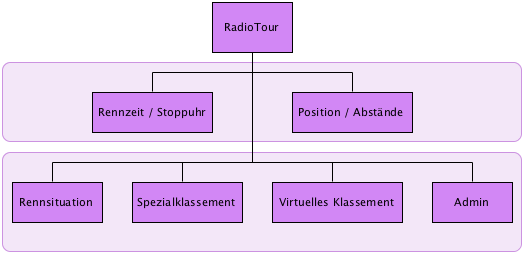
\includegraphics[scale=0.9]{05bericht/images/struktur.png}
\end{figure} 

Der Stamm stellt die Applikation dar und die Äste zeigen die Aufteilung der Funktionen. Die Rennzeit sowie die aktuelle Rennposition sind in einem immer sichtbaren Bereich platziert.
\\
Die untere Ebene beinhaltet die Kernelemente der Applikation. Diese werden in Views seitenweise dargestellt. Durch eine Navigation lässt sich zwischen den Views wechseln, ohne dass dabei die Live Informationen ausgeblendet werden.

\section{Schichtenmodell und Paketdiagramm}
Die Applikation lässt sich in vier verschiedene Schichten aufteilen. Diese Schichten sind in der folgenden Grafik illustriert. Die oberste Schicht stellt dabei die Schnittstelle zum Benutzer dar. Innerhalb der Schicht werden die dabei verwendeten Pakete angezeigt.  
\begin{figure}[h!]
\caption{Die Schichten der Applikation inklusive der verwendeten Pakete}
\label{fig:layer}
\centering
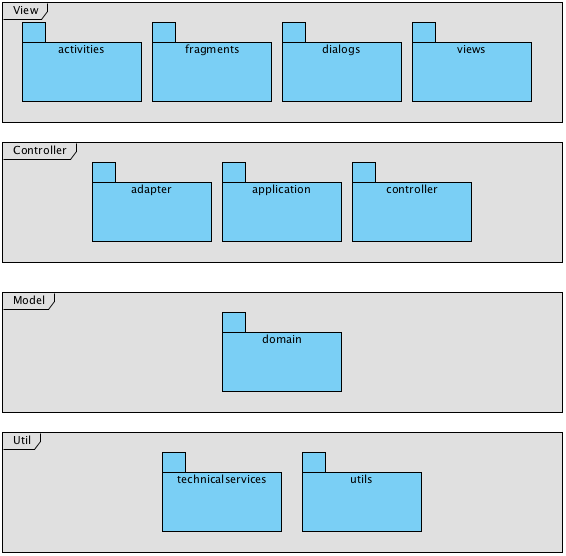
\includegraphics[scale=0.9]{05bericht/images/packagediagram.png}
\end{figure} 

Die \textit{View} Schicht in der Abbildung \ref{fig:layer} enthält alle Pakete in welchen Elemente zur Benutzerinteraktion definiert sind. Um die einzelnen Pakete in dieser Schicht zu verstehen, wird hier ein kurzer Exkurs zu Android View Elementen eingeschoben. Für die Elemente \textit{Activity} und \textit{Fragment} wird hierfür ein Teil der Android \gls{api} Beschreibung zitiert.

\begin{quote}
\textit{An Activity is an application component that provides a screen with which users can interact in order to do something, such as dial the phone, take a photo, send an email, or view a map. Each activity is given a window in which to draw its user interface. The window typically fills the screen, but may be smaller than the screen and float on top of other windows.}\footnote{Android Developers Reference, \url{http://developer.android.com/guide/topics/fundamentals/activities.html}, aufgerufen am 31.05.2012.}
\end{quote}

Die \textit{RadioTour} Applikation besteht aus einer Activity. Dies aus der Entscheidung heraus, dass gewisse Inhalte, wie zum Beispiel die aktuelle Etappe oder die Stoppuhr jederzeit verfügbar sein müssen. Diese Activity befindet sich im Paket \textit{activities}

\begin{quote}
\textit{A Fragment represents a behavior or a portion of user interface in an Activity. You can combine multiple fragments in a single activity to build a multi-pane UI and reuse a fragment in multiple activities. You can think of a fragment as a modular section of an activity, which has its own lifecycle, receives its own input events, and which you can add or remove while the activity is running (sort of like a "`sub activity"' that you can reuse in different activities).}\footnote{Android Developers Reference, \url{http://developer.android.com/guide/topics/fundamentals/fragments.html}, aufgerufen am 31.05.2012.}
\end{quote}

Eine spezielle Form der Fragmente stellen DialogFragmente dar. Sie werden benutzt um einen Dialog über der Activity einzublenden. In der Applikation werden diese Elemente verwendet um Daten zu erfassen und zu ändern. Die DialogFragmente der Applikation befinden sich im Paket \textit{dialogs}.

Für eine genauere Analyse der in der \textit{View} Schicht verwendeten Elemente und Klassen sei auf das Kapitel \ref{ref:realisierung} verwiesen.
\\
Die \textit{Controller} Schicht in der Abbildung \ref{fig:layer} ist für die Aufbereitung der Daten welche von der \textit{View} Schicht dargestellt wird verantwortlich.

Die \textit{Model} Schicht in der Abbildung \ref{fig:layer} stellt die Daten Objekte für die Applikation zur Verfügung. Eine Darstellung der in der \textit{RadioTour} App  verwendeten Domain Objekte ist in der Abbildung \ref{fig:domain} ersichtlich.

Die \textit{Util} Schicht in der Abbildung \ref{fig:layer} beinhaltet die Dienstobjekte für den Datenbank Zugriff sowie für die Kommunikation der Applikation mit dem cnlab Server. Im Paket \textit{utils} befinden sich allgemein gebrauchte Hilfsmethoden.


\section{Klassendiagramm}
Die Domainlogik beinhaltet die Kernelemente der Applikation. Einerseits sind dies die Rennfahrer, welche Informationen über sich festhalten, andererseits die Etappe mit den Informationen zur Strecke. Während dem Rennen werden die Fahrer in Gruppen unterteilt. Auch diese Gruppen sind in der Domain abgebildet. Das Klassendiagramm des Domain Package zeigt die wesentlichen Elemente.

\begin{figure}[h!]
\caption{Die Domainklassen in der Abhängigkeit}
\label{fig:domain}
\centering
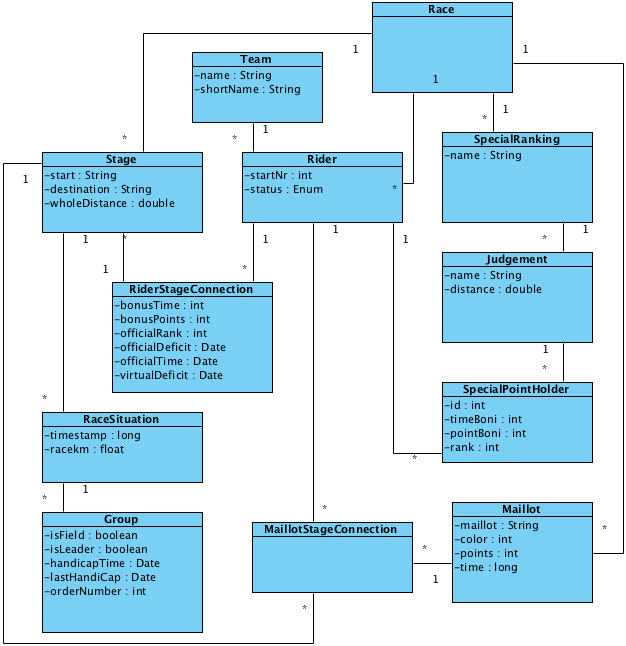
\includegraphics[scale=0.8]{05bericht/images/domain.png}
\end{figure} 


Die Klasse \textit{Rider} speichert die Angaben zu einem Fahrer und beinhaltet keine eigene Logik. Objekte dieser Klasse dienen als Stammdaten für alle Etappen welche in der Applikation erfasst sind.\\
Um die Fahrer nach Team sortiert anzeigen zu können, wird die Klasse \textit{Team} genutzt.\\
In \textit{Stage} ist die Etappe definiert. Jede Etappe hat eine Marschtabelle in Form von mehreren \textit{PointOfRace} Objekten. Diese Objekte werden durch Import der Marschtabelle erstellt.\\
Da pro Etappe jeder \textit{Rider} einen anderen \textit{RiderState} haben kann, gibt es die Verbindungsklasse \textit{RiderStageConnection}. In dieser Klasse ist jeweils die Etappe mit dem Fahrer verknüpft. Dies ermöglicht es, den Rückstand eines Fahrers in mehreren Etappen differenziert zu verfolgen. Dadurch werden bei einem Etappenwechsel innerhalb der Applikation immer die Informationen zur ausgewählten Etappe verwendet.\\
Die Klasse \textit{SpecialRanking} stellt ein Spezialklassement dar und wird benötigt, um die einzelnen Wertungen (\textit{Judgement}), welche Etappen basiert sind, auch über alle Etappen hinweg zu verrechnen. Damit können zum einen Punkte- bzw. Zeitboni pro Etappe verrechnet werden, was zur Darstellung im Virtuellen Klassement gebraucht wird und zum andern eine Rangliste pro Spezialklassement geführt werden. Diese Rangliste enthält die Ergebnisse aller Wertungen des angegebenen Spezialklassements ohne Rücksicht auf die zugehörige Etappe.\\
Die \textit{SpecialPointHolder} Klasse dient dazu, den zu Wertungen zugewiesenen Fahrern in der Datenbank zu speichern und zur späteren Berechnung des virtuellen Klassements berücksichtigen.\\
Eine \textit{RaceSituation} stellt einen Stand von \textit{Group} Objekten zu einem speziellen Zeitpunkt und Kilometerstand dar. Objekte vom Typ \textit{RaceSituation} werden bei jeder Neugruppierung von Fahrern oder Setzen eines Rückstandes einer Gruppe erstellt, an den Server gesendet und in die lokale \gls{sqlite} Datenbank geschrieben. Jeweils beim Start der Applikation sowie beim Wechseln der aktuellen Etappe wird die zuletzt in der Datenbank abgespeicherte \textit{RaceSituation} geladen. Die \textit{Group} Klasse enthält die Angaben zum aktuellen Rückstand zur Spitze, dem letzten bekannten Rückstand sowie boolsche Attribute welche bestimmen ob die Gruppe das Feld oder die Spitze darstellt.\\
Mit Hilfe der \textit{Maillot} Klasse können Maillots erstellt und verteilt werden, welche dann über alle Etappen bestehen. Da nach jeder Etappe ein anderer Fahrer ein Maillot tragen kann, wird eine Verbindung zwischen der Etappe und einem Maillot gebraucht. Diese Funktion wird durch die Klasse \textit{MaillotStageConnection} erfüllt. 


\section{Datenbankschema}
Die Nutzung von ORMLite zur Objektrelationalen Abbildung von Instanzen in die \gls{sqlite} Datenbank impliziert, dass das Datenbankschema der Klassenstruktur wie in \ref{fig:domain} abgebildet entspricht. 

\section{Sequenz Diagramm}
Der häufigste UseCase besteht darin, die Rennsituation zu erfassen und an den Server zu übermitteln. Gleichzeitig werden im Hintergrund die Live Informationen aktualisiert. Diese beiden Hauptanwendungsfälle sind im folgenden System Sequenz Diagramm dargestellt. Der Actor wird durch den \textit{RadioTour Speaker} dargestellt und das System durch die \textit{RadioTour} Applikation. Das externe System stellt die Serverseite dar.

\begin{figure}[h!]
\caption{Das System Sequenz Diagramm}
\label{fig:ssd_rennen}
\centering
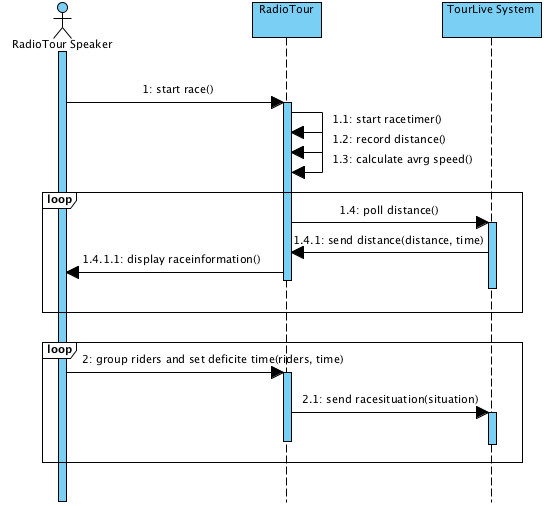
\includegraphics[scale=0.9]{05bericht/images/ssd_rennen.png}
\end{figure} 

Das Rennen wird durch das Starten der Rennzeit gestartet. Ab diesem Zeitpunkt beginnt die Aufzeichnung des Rennkilometers und die Berechnung der durchschnittlichen Geschwindigkeit.